\subsection{VERSO}
\label{sec:verso}

The software residing on the DAQ PC or server side of the VRS system,
illustrated in Figure~\ref{fig:vrs_diagram_minimal} and \ref{fig:vrs_diagram},
provides the main interface by which users can control the overall
state of the frontend electronics, either on- or off-detector,
as well as control the data acquisition and monitoring.
The high-level software suite containing these functionalities is referred
to as \textit{VERSO}, an acronym for `VMM Embedded ReadOut Software'.
In this section an overview of VERSO's role within the VRS system will be provided.

The user interface and software backend to VERSO are written entirely in C++,
with the user interface relying primarily on the Qt framework~\cite{QtCompany}.
The VERSO user interface is shown in Figure~\ref{fig:verso_main}.
VERSO has two main responsibilities: orchestrating configuration processes and
data-acquisition (DAQ).
Both functionalities are performed using a custom-made communication protocol
implemented in the UDP/IP communication protocol.
As illustrated in Figures~\ref{fig:vrs_diagram_minimal} and \ref{fig:vrs_diagram},
all communication from VERSO is sent over the network to either FPGAs located directly
on the frontend boards or on the VRS supervisory board, depending on the
data-taking situation.
The logical blocks indicated in Figure~\ref{fig:verso_main} are described as follows:

\begin{description}
    \item[] \textbf{Run Control} This block sets up the underlying configuration and DAQ
        that VERSO implements.
        From here the user can initiate and terminate the data taking sessions (`runs').
        VERSO supports several frontend types, either differing in the version of the VMM or in the
            implementation of the firmware (selected by the `VMM2', `VMM3', or `L0 R/O' buttons).
        The `Setup' and `Config' fields allow a user to load configuration files describing
            the detector-readout-element-to-VMM-channel mapping and VMM ASIC configuration, respectively.\footnote{
                The detector-readout-element-to-VMM-channel mapping refers to both the geometric description
                of any detectors to which VERSO is communicating and the correspondence, for example, between an MM detector's
                strip location to the frontend board and VMM channel responsible for reading out that MM strip's signals.
                This correspondence is required if one wishes to construct high level objects, such as
                particle tracks, traversing through several detector layers and with each layer read out
                by different frontend boards.
            }
    \item[] \textbf{Network Communication} This block describes the network addresses of the
        frontend electronics and handles the sustained connection to them.
    \item[] \textbf{FPGA and Operational Parameters} This block sets the configuration parameters
            for the FPGA on the connected frontend boards. Such parameters, for example,
            are the frequency and width of the VMM channel test pulse signal and the bunch
            crossing clock driving the readout of the VMM ASIC.
    \item[] \textbf{Message Reporting} Reports messages visually so that the user may acknowledge
            the current state of the system. Sends messages also to files.
    \item[] \textbf{VMM Configuration Panel} The `Global Registers' and `Channel Registers' panels allow
        the user to set the configuration parameters of the VMM ASICs on the frontend boards.
        An instance of the VMM Channel Registers panel is shown in Figure~\ref{fig:verso_chanreg}.
    \item[] \textbf{VMM Calibration Panel} This panel allows the user to schedule various calibration routines.
        The user may also provide files containing calibration constants/parameters, derived from previous
        calibration runs, that get loaded into the associated VMM configuration
        bitstreams during the VMM configuration process.
\end{description}

\noindent The configuration of the FPGA is sent over the network from VERSO and
follows an address-value mechanism whereby each configurable parameter of the FPGA has its
value stored within the FPGA at a specific memory register.
VERSO sets an FPGA configurable parameter by forwarding a register address followed by its corresponding
value set on the user interface.
The FPGA sends acknowledgement packets over the network to VERSO upon each message received,
indicating whether it was able to successfully perform the requested configuration action or not.
If not, then VERSO can log this information and can re-attempt transmission of the lost or mis-handled packet
containing the configuration specification.
%The configuration of the VMM ASICs is forwarded by the FPGA via the Serial Peripheral Interface (SPI) protocal
%to the VMMs.
The VMM ASIC recieves its own configuration following a Serial Peripheral Interface (SPI) protocol.
An individual VMM ASIC configuration is rather large, given its highly configurable nature, and is
nearly 2 kilobits long.
The specification of the configuration bitstreams is specified by the user in the `Global' and `Channel' configuration
panels on the user interface, shown in Figure~\ref{fig:verso_main}.
The `Global' VMM parameters are those that are not specific to an individual channel; for example,
the VMM channel threshold, channel gain, or the specification of the VMM shaper integration time.
The VERSO software handles the construction of the configuration bitstreams for each VMM ASIC and forwards
them to the corresponding FPGA housing the VMM to be configured.
Upon receipt of a VMM configuration bitstream, the FPGA forwards it to the SPI input of the specified VMM.
The FPGA knows to which of the (potentially several) on-board VMMs to forward the configuration based on
a custom addressing dataframe parsed by the FPGA that VERSO prepends to each configuration bitstream.


\begin{figure}[!htb]
    \begin{center}
        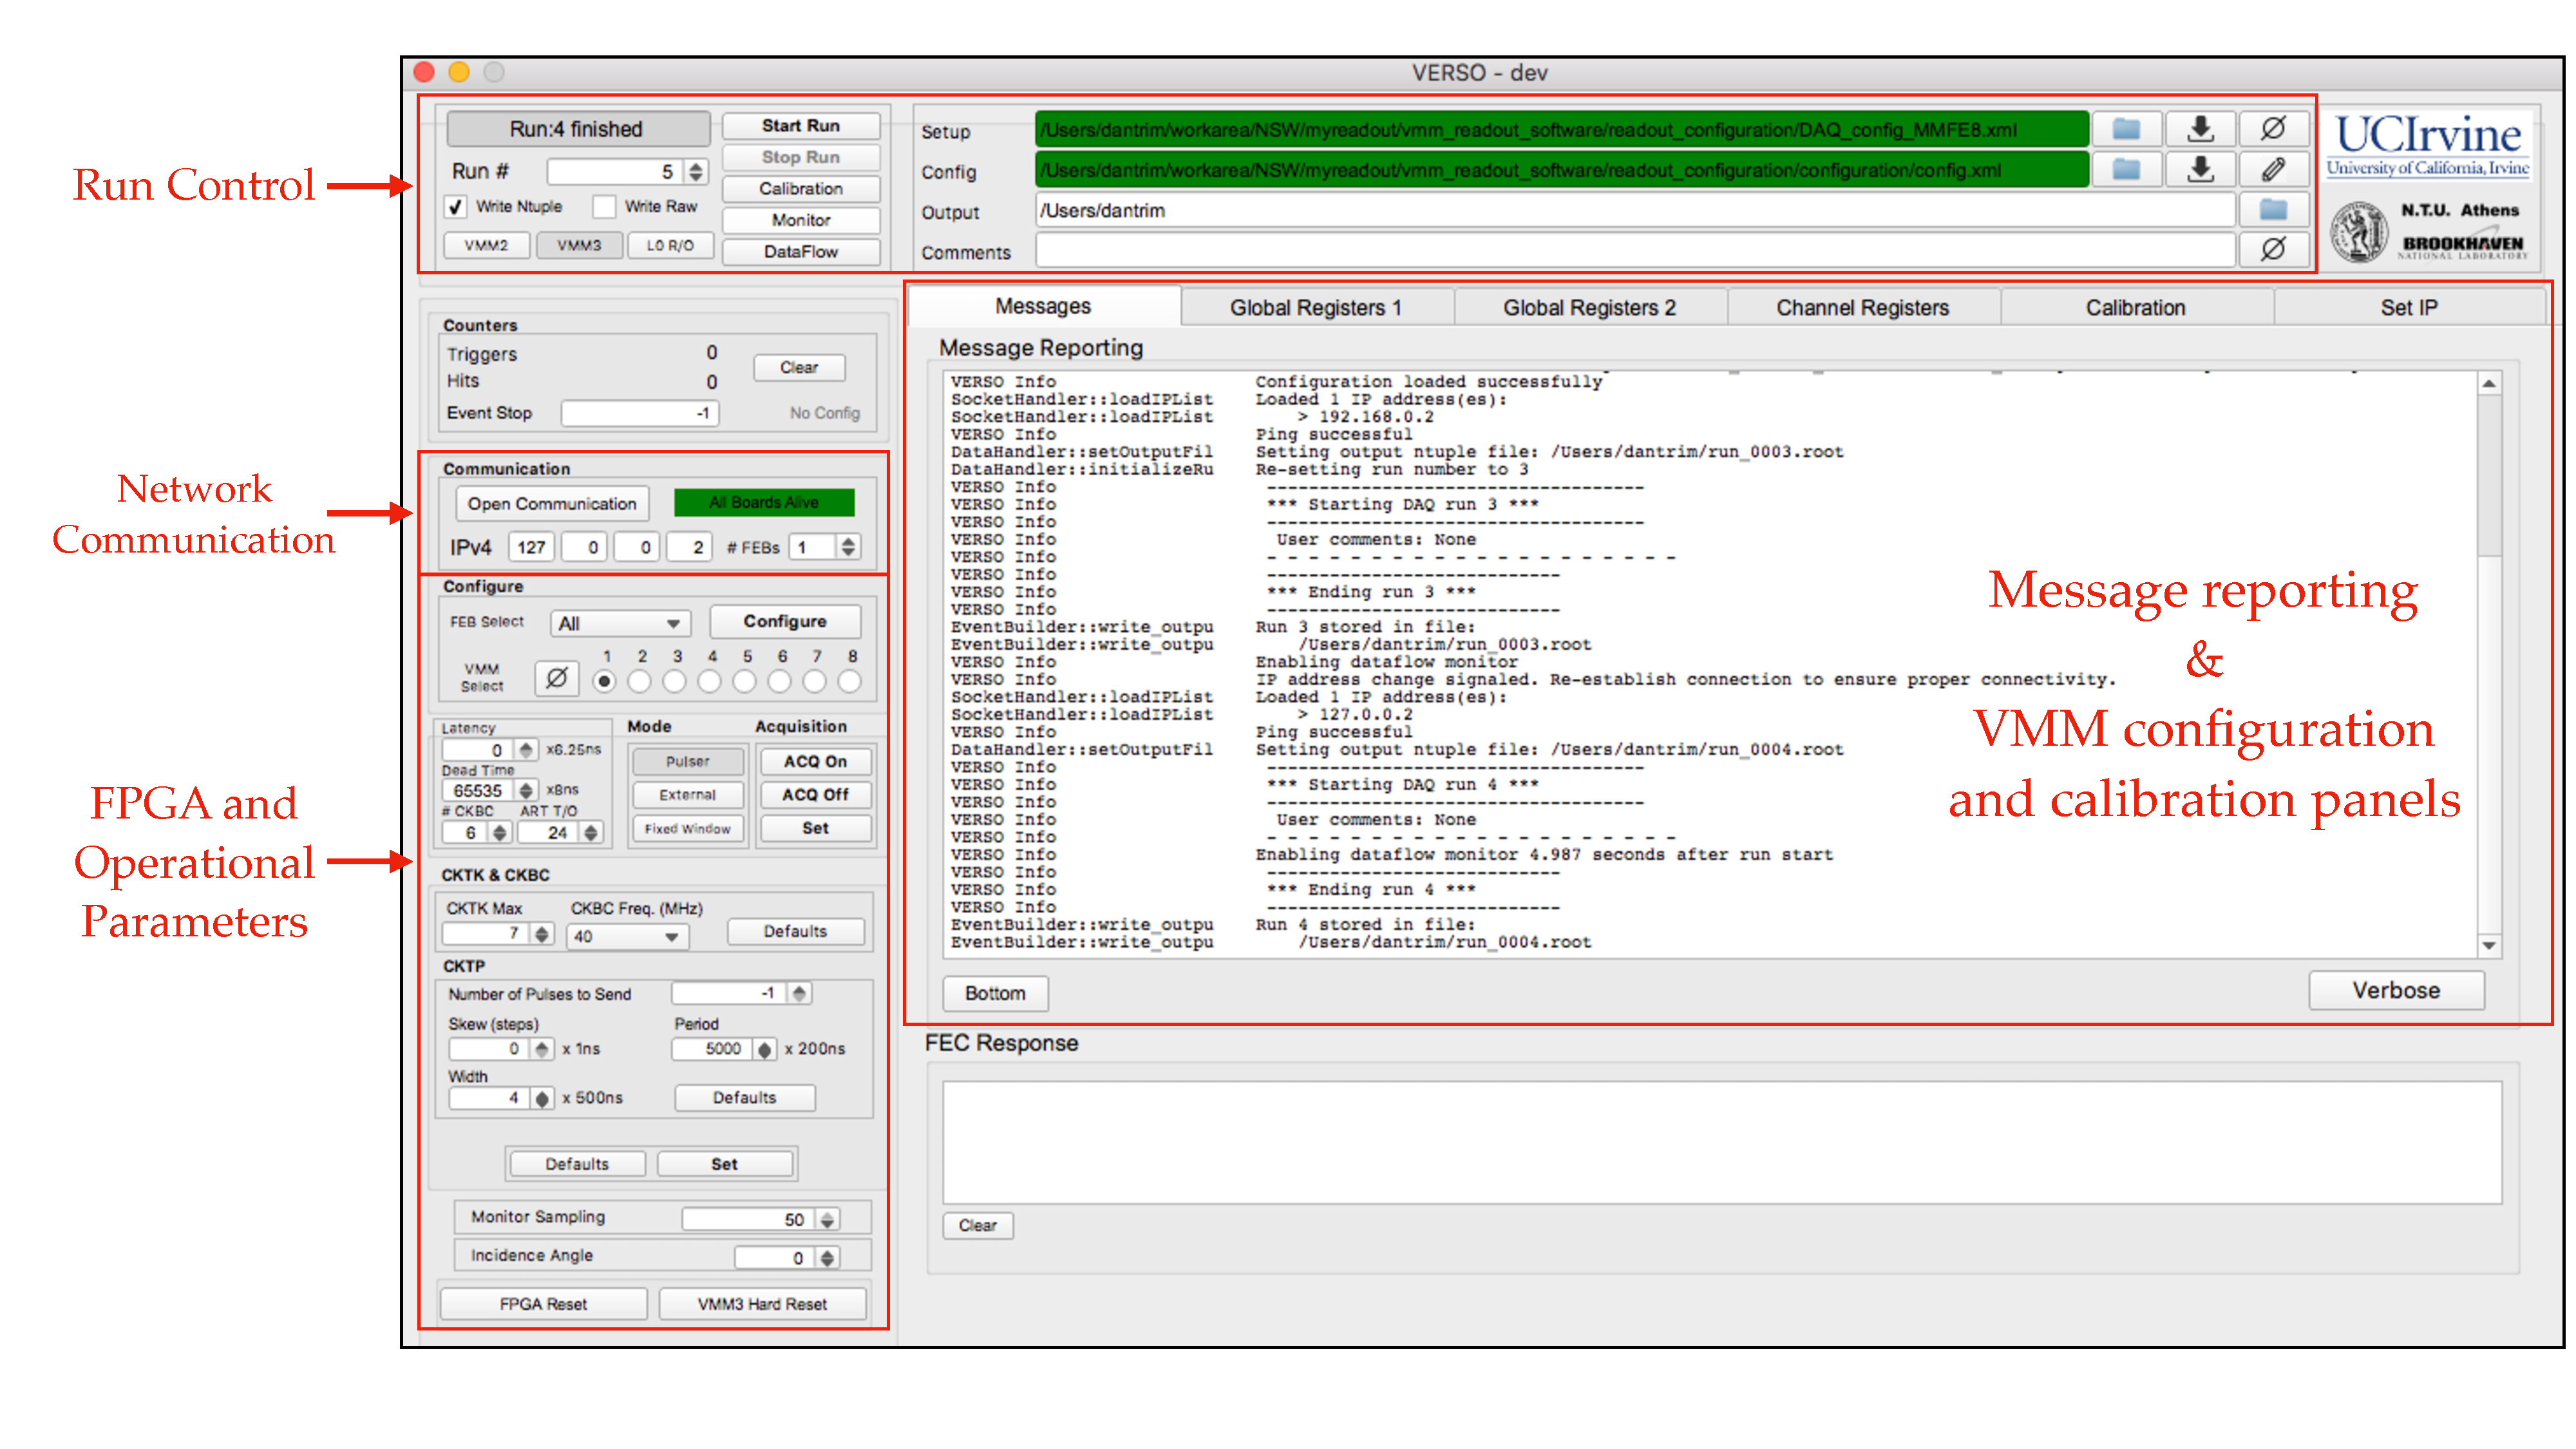
\includegraphics[width=0.95\textwidth]{figures/nsw/vrs/verso_mainPDF}
        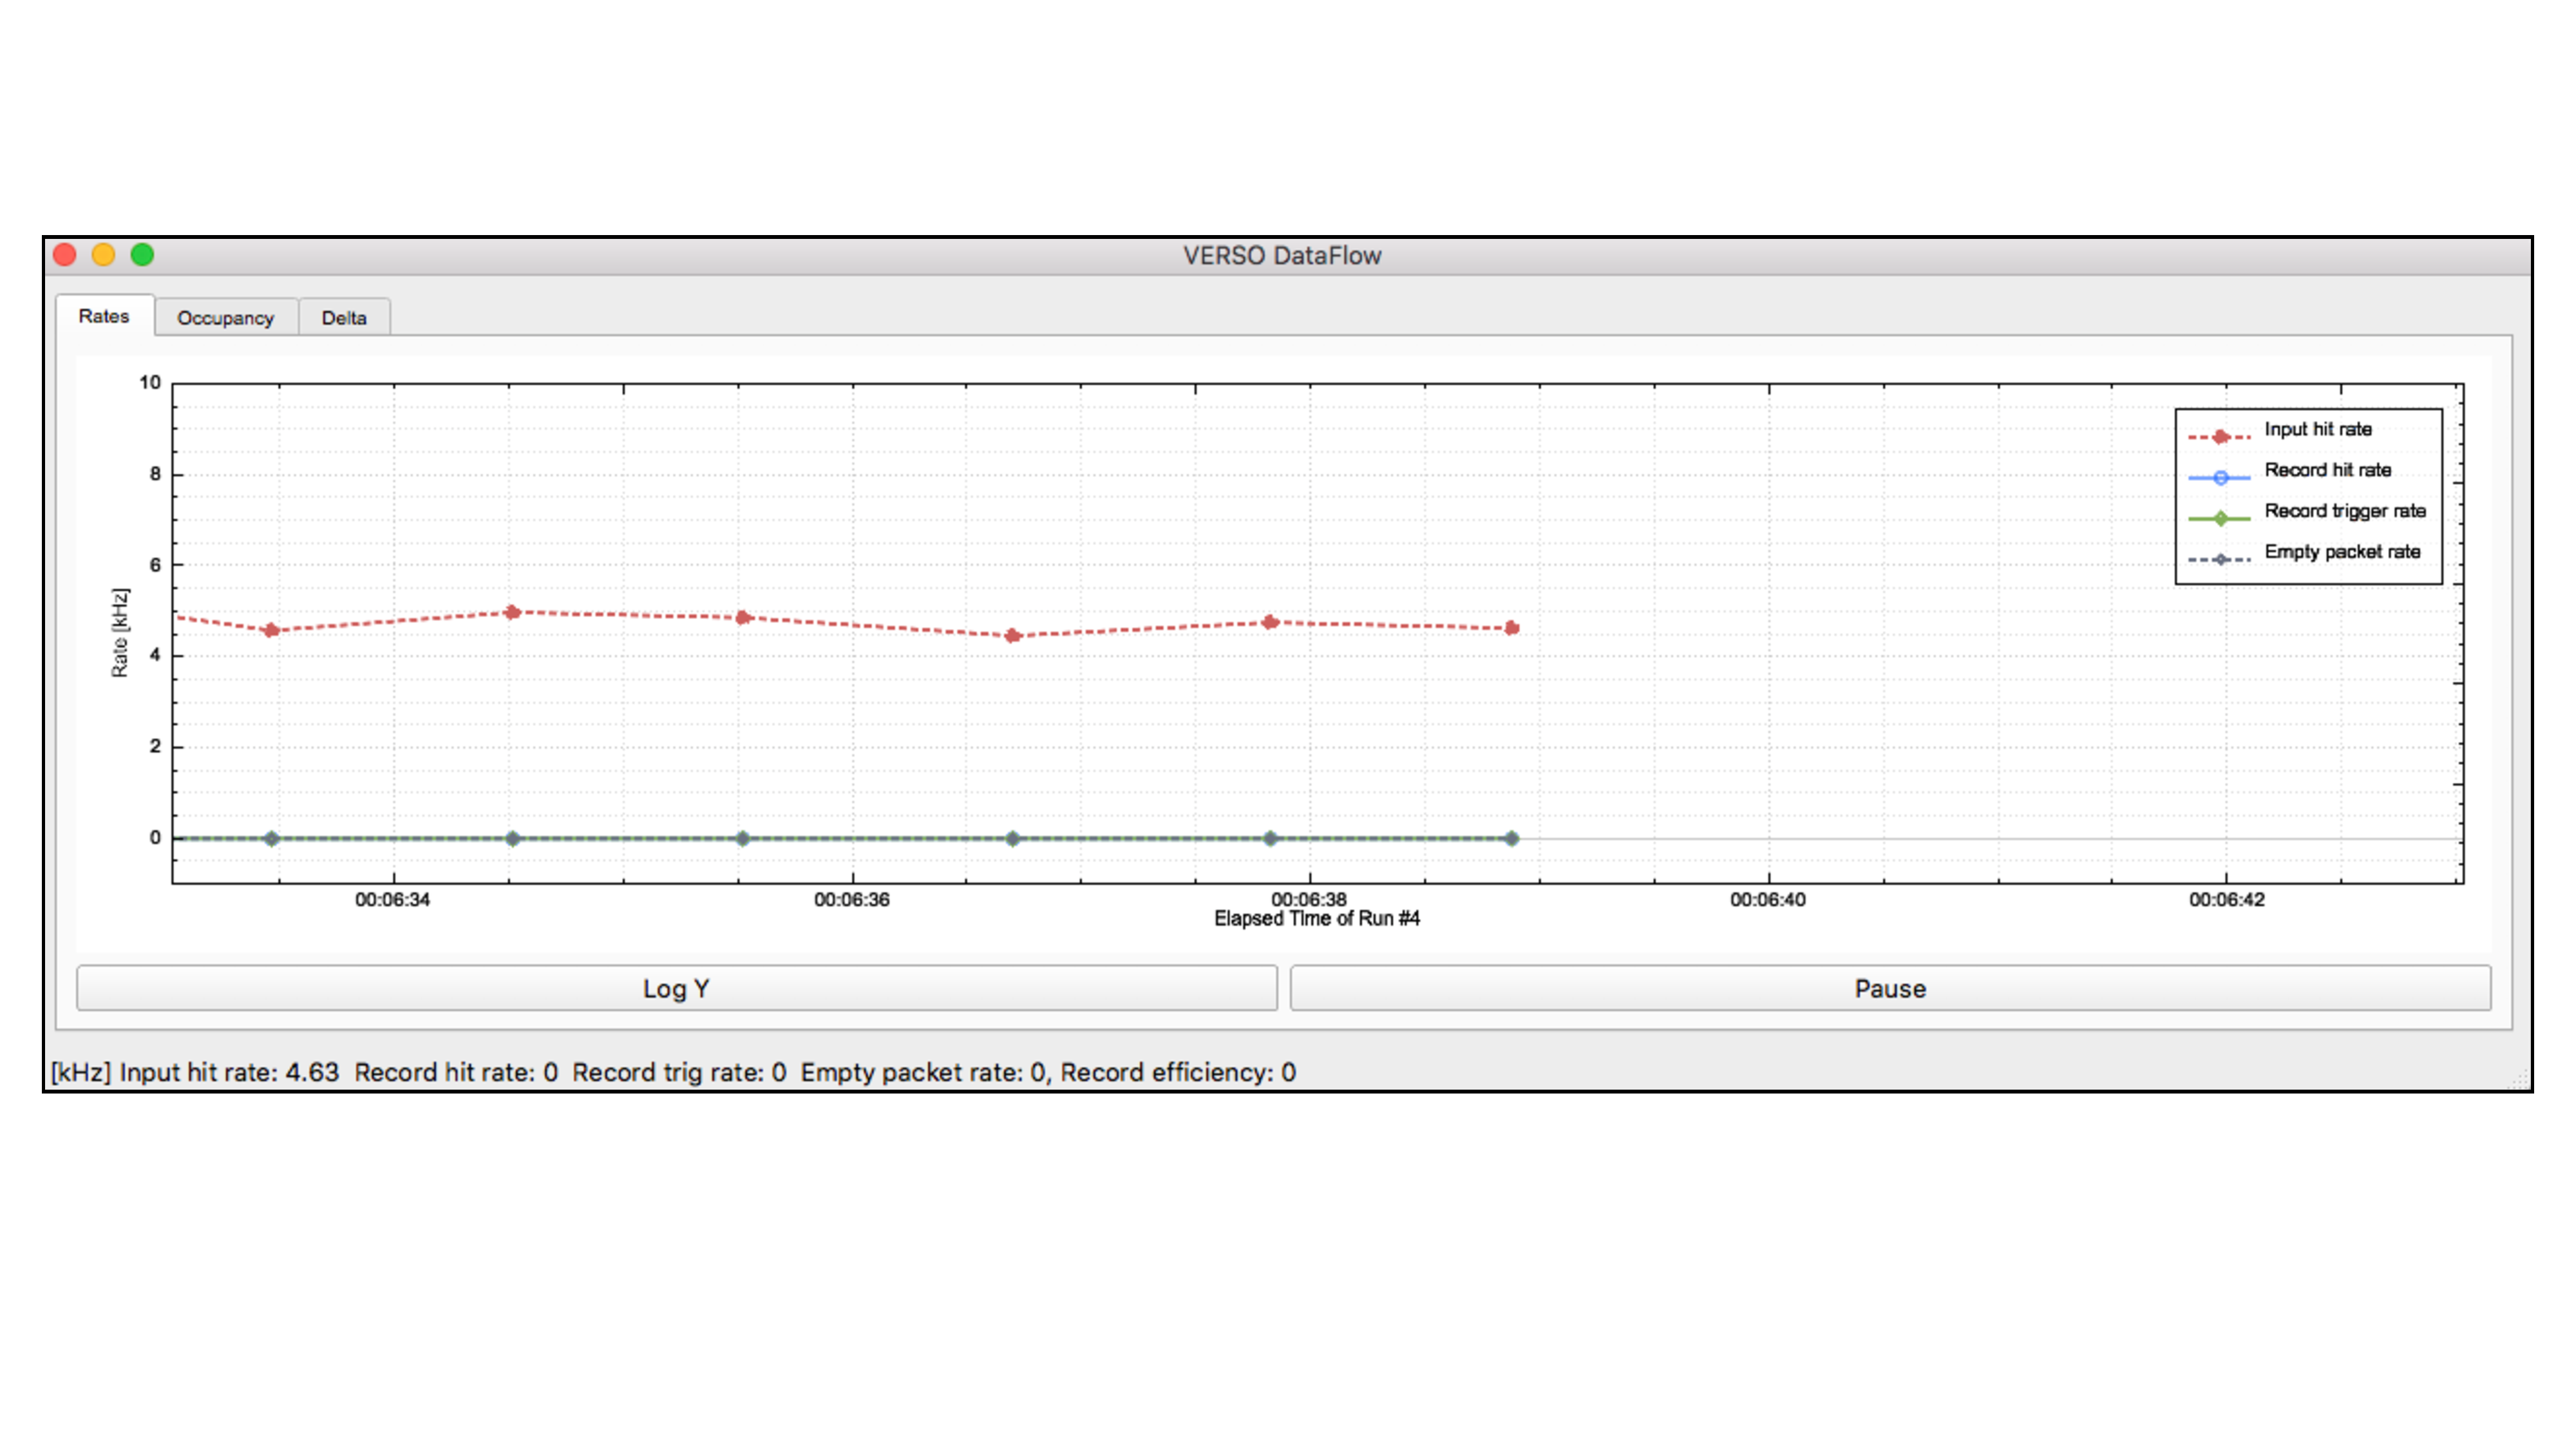
\includegraphics[width=0.8\textwidth]{figures/nsw/vrs/verso_dataflow}
        \caption{
            \textbf{\textit{Top}}: Main VERSO user interface, with different logical blocks indicated.
            \textbf{\textit{Bottom}}: VERSO dataflow monitor, showing the rate of VMM channel hits
                for all connected frontend boards and VMMs. Also displayed are the rate at which individual
                hits and events are recorded, where an `event' is a collection of hits associated with the
                same trigger.
                The data being shown in this graph correspond to hits generated with the VMM channel
                test pulse injection with the output data recording disabled.
                The DAQ efficiency, during a normal data taking period with recording enabled, is defined
                as the number of recorded VMM hits divided by the number of input VMM hits having been
                sent from the frontend electronics.
        }
        \label{fig:verso_main}
    \end{center}
\end{figure}

\begin{figure}[!htb]
    \begin{center}
        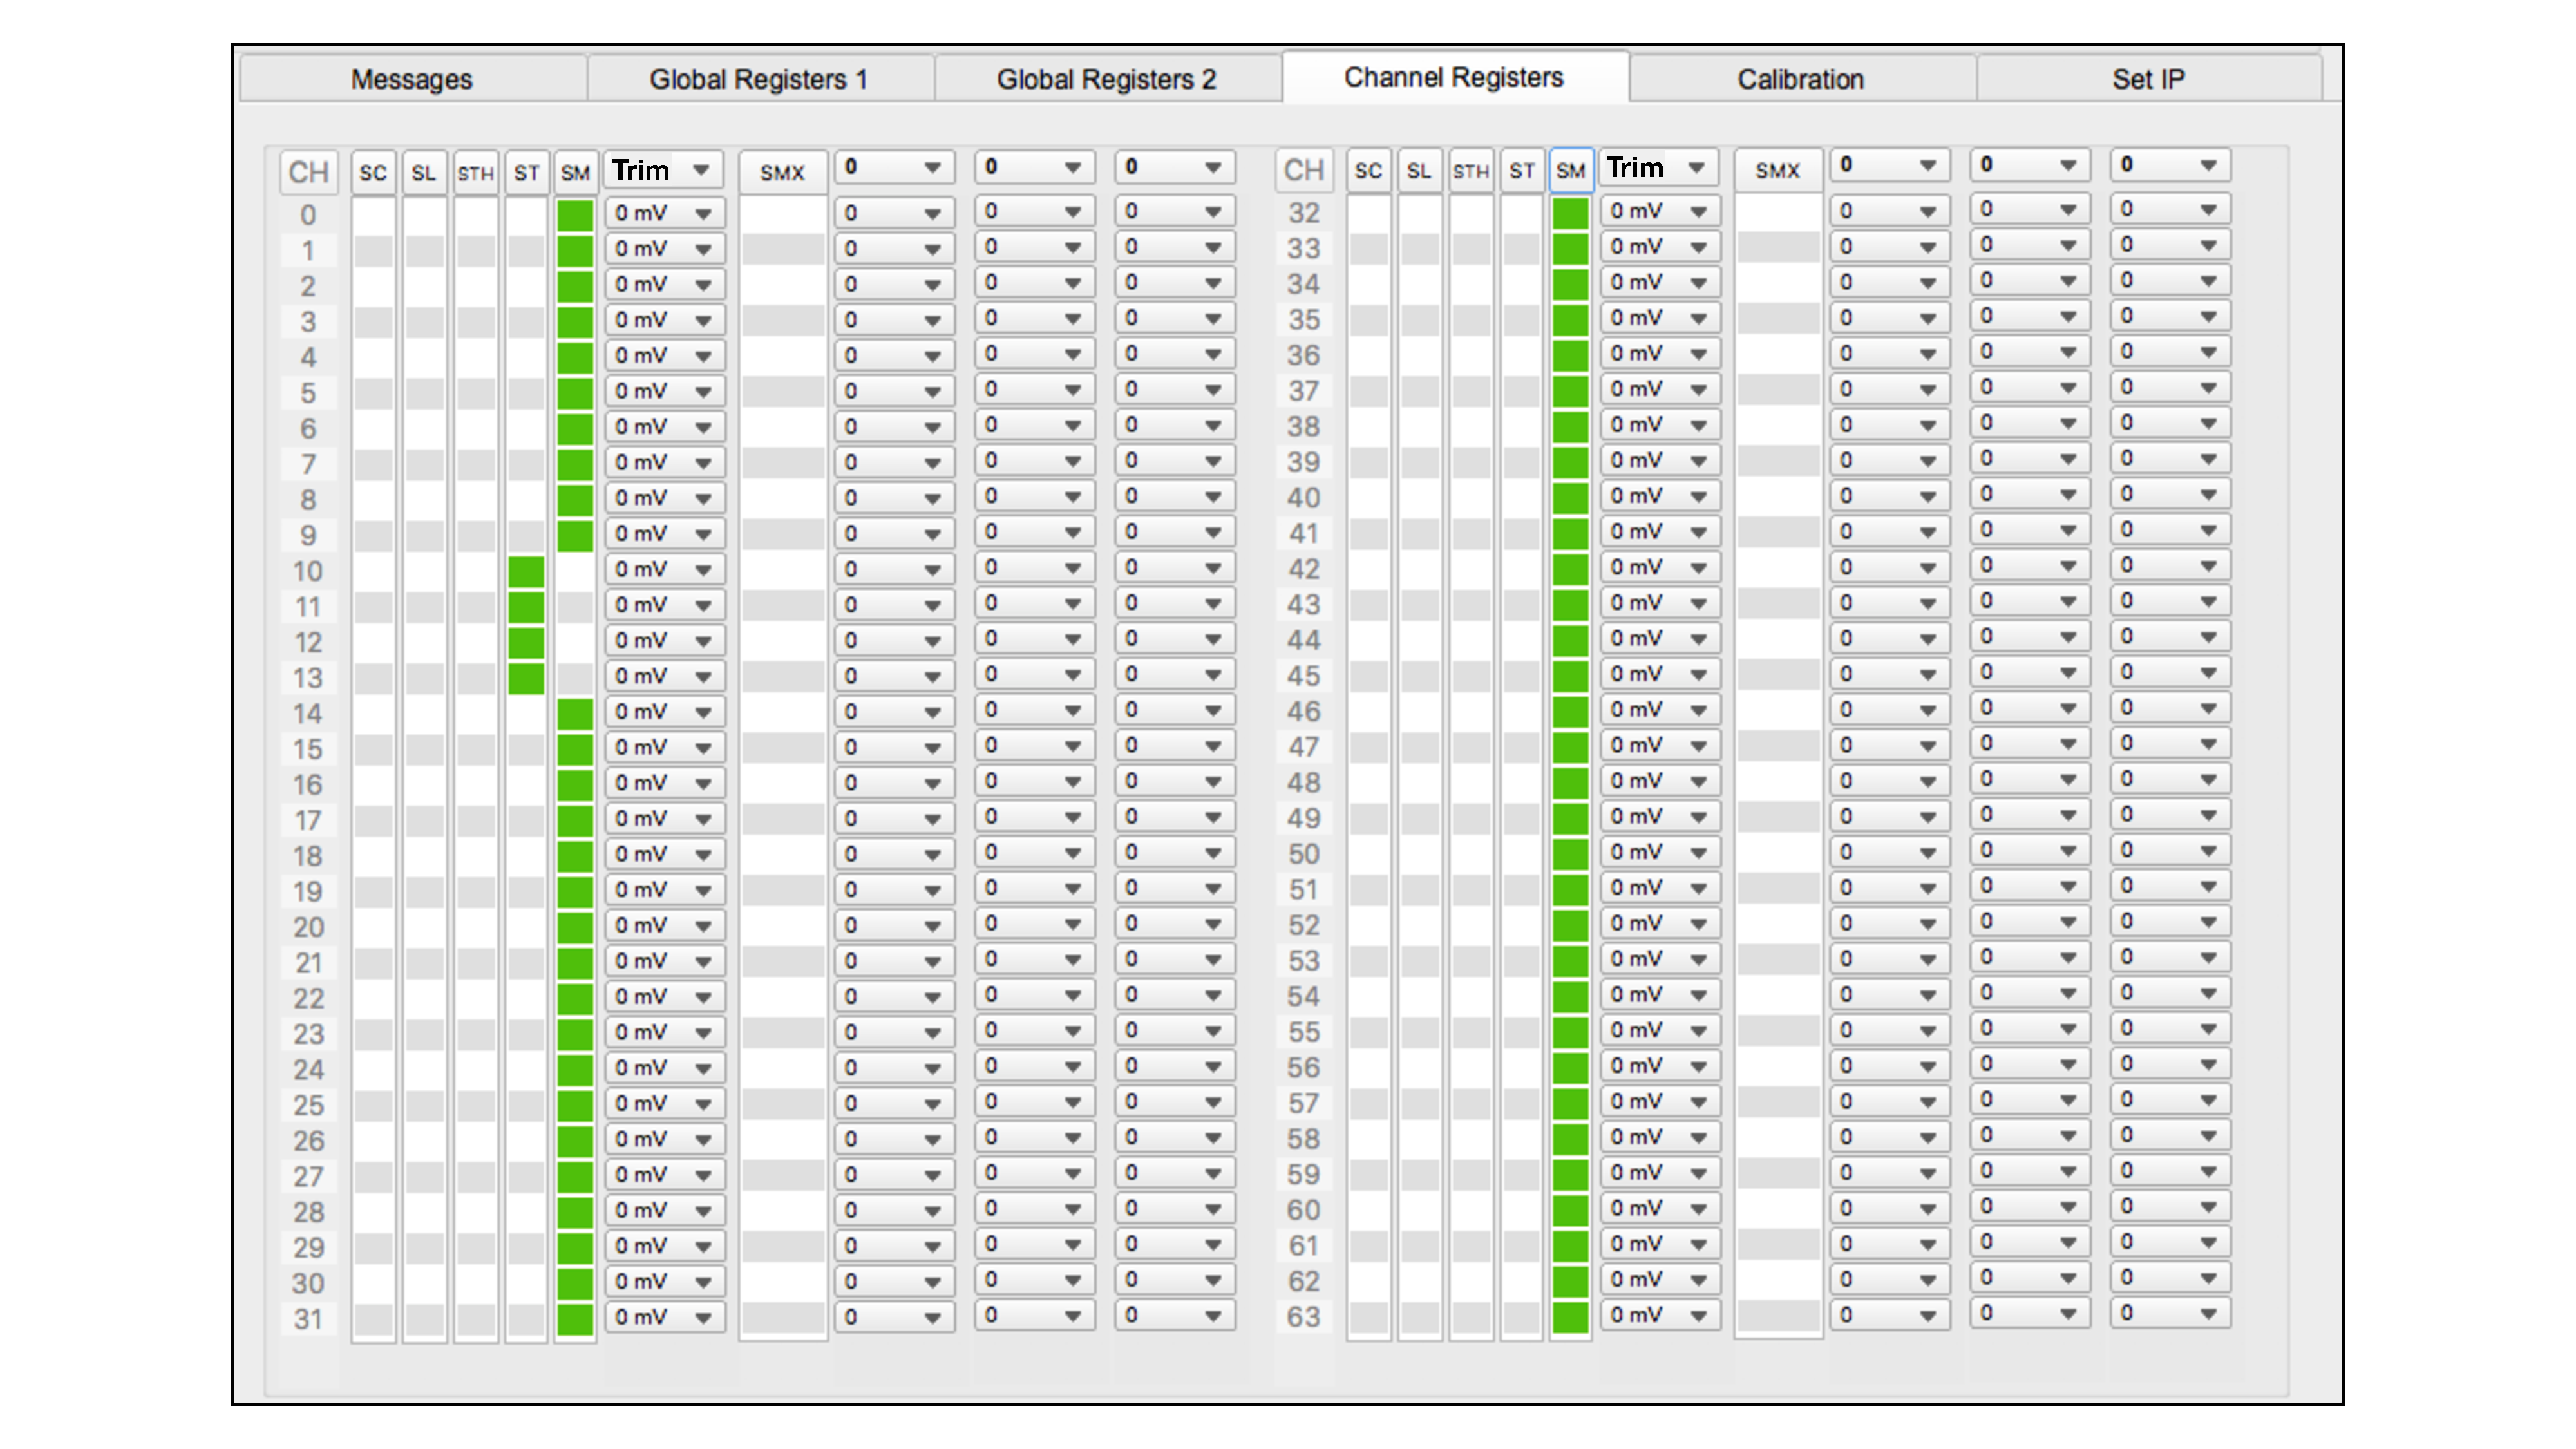
\includegraphics[width=0.8\textwidth]{figures/nsw/vrs/verso_chanreg}
        \caption{
            The VERSO `Channel Registers' panel, showing the configuration specification
            of each of the 64 channels of an individual VMM.
            The `ST' (`SM') flags activate the corresonding channel's internal test-charge
            capacitor (masking).
            In the example shown, VMM channels 10-13 (inclusive) will have their
            test-charge capacitor activated. All other channels are masked and
            are effectively disabled.
            The `Trim' configuration refers to the 5-bit channel threshold trimming,
            specifying by how much the individual channel's threshold should be moved
            relative to the global VMM threshold value.
        }
        \label{fig:verso_chanreg}
    \end{center}
\end{figure}

The VERSO DAQ backend is responsible for handing the readout of the frontend boards.
VMM hit data is sent over the network and received by VERSO.
The hit data may be that of a detector being readout by the VMM-based frontend electronics
or simulated data created by the VMM channel test-charge capacitors that can inject
signal onto each of the VMM channel inputs.
In the latter case, the frequency and characteristics (width, amplitude, etc...) of the
signals are specified via the FPGA configuration described above, since the FPGA orchestrates
the triggering of the VMM channel test-charge injection signals.

VERSO's DAQ functionalities are implemented following a single-producer/single-consumer
architecture.
In such an architecture, at the start of each run, the software constructs two threads with independent
tasks.
One thread is responsible for receiving the raw data packets over the network from the
frontend electronics and subsequently buffering them in a queue.
The data fragments received over the network are indexed in this queue by their corresonding
event or trigger identifier: VMM hit data corresponding to a single trigger will all be given the
same such identifier.
The second thread is responsible for taking all the data fragments received for each corresponding
trigger, decoding and inspecting the raw data contained therein, and building output
data fragments that represent high level constructs that associate the VMM hits
with specicific frontend boards and/or detector readout elements.
This latter aspect --- the gathering together of all data fragments corresponding to a
specific trigger --- is referred to as `event building'.
Once an event is built, VERSO stores it on disk in the ROOT \texttt{TTree} format
for later analysis.

Given the asynchronous nature of the network communication, as well as the fact that the UDP/IP
network protocol does not ensure a fixed latency, events based on the same trigger
are not guaranteed to be captured by VERSO within the same UDP/IP network packet.
The use of the single-producer/single-consumer model is adapted to such a case, with
the producer thread indexing and filling the queue and the consumer thread performing the event building.
In VERSO, the queue in which indexed data fragments are stored is implemented
as a lock-free, concurrent queue.
As a result, the queue may be accessed and manipulated by each thread without affecting or blocking
the other, allowing for smooth DAQ operation.
The event building thread can then periodically inspect the queue and wait for a configurable amount of time for the expected
number of data fragments from each of the frontend elements before finishing
the event building process.
Once the event building process is completed,
the event building thread starts the process over and begins gathering the data fragments from the next-received trigger number identifier.
The use of the multi-threaded architecture, pivoting around a fast concurrent queue, has allowed VERSO to achieve 100\% DAQ efficiency
in all use-cases encountered ({\color{red}{Section XXX for use-cases}}).



\FloatBarrier
